\documentclass[landscape,a2paper,fontscale=0.65]{baposter}

\usepackage{multicol} % This is so we can have multiple columns of text side-by-side
\columnsep=100pt % This is the amount of white space between the columns in the poster
\columnseprule=3pt % This is the thickness of the black line between the columns in the poster

%\usepackage{times} % Use the times font
%\usepackage{palatino} % Uncomment to use the Palatino font
\usepackage{kpfonts, baskervald}

\usepackage{graphicx} % Required for including images
\usepackage{booktabs} % Top and bottom rules for table
\usepackage[font=small,labelfont=bf]{caption} % Required for specifying captions to tables and figures
\usepackage{amsfonts, amsmath, amsthm, amssymb} % For math fonts, symbols and environments
\usepackage{wrapfig} % Allows wrapping text around tables and figures
\usepackage{graphicx,caption,float}
\usepackage{bbm}
\usepackage{bbold}
\usepackage{amsthm}
\usepackage{amsmath}
\usepackage{xcolor}
\usepackage{url,hyperref}
\usepackage[none]{hyphenat}
\usepackage{amssymb}
\usepackage{amsfonts}
\usepackage{listings}
\usepackage{mwe}
\usepackage[toc,page]{appendix}
\usepackage{enumitem}
\usepackage[noend]{algpseudocode}
\usepackage[english]{babel}
\usepackage[utf8]{inputenc}
\usepackage{listings}
\newtheorem{theorem}{Theorem}
\usepackage{color}
\usepackage{subfig}
\usepackage{multirow}
\usepackage{array}
\usepackage{mathtools}

\usepackage{pifont}
\renewcommand{\labelitemi}{\ding{229}}
\renewcommand{\labelitemii}{\ding{228}}
\renewcommand{\labelitemiii}{\ding{225}}

\setlength\floatsep{0pt}
\setlength\textfloatsep{0pt}
\setlength\intextsep{0pt}
\setlength{\belowdisplayskip}{0pt} \setlength{\belowdisplayshortskip}{0pt}
\setlength{\abovedisplayskip}{0pt} \setlength{\abovedisplayshortskip}{0pt}

\graphicspath{{images/}}
\usepackage{etoolbox}
\patchcmd{\thebibliography}{\section*{\refname}}{}{}{}

\begin{document}
%% Format it to your taste with the options
\background{
      \begin{tikzpicture}[remember picture,overlay]%
      \draw (current page.north west)+(-2em,2em) node[anchor=north west]
      {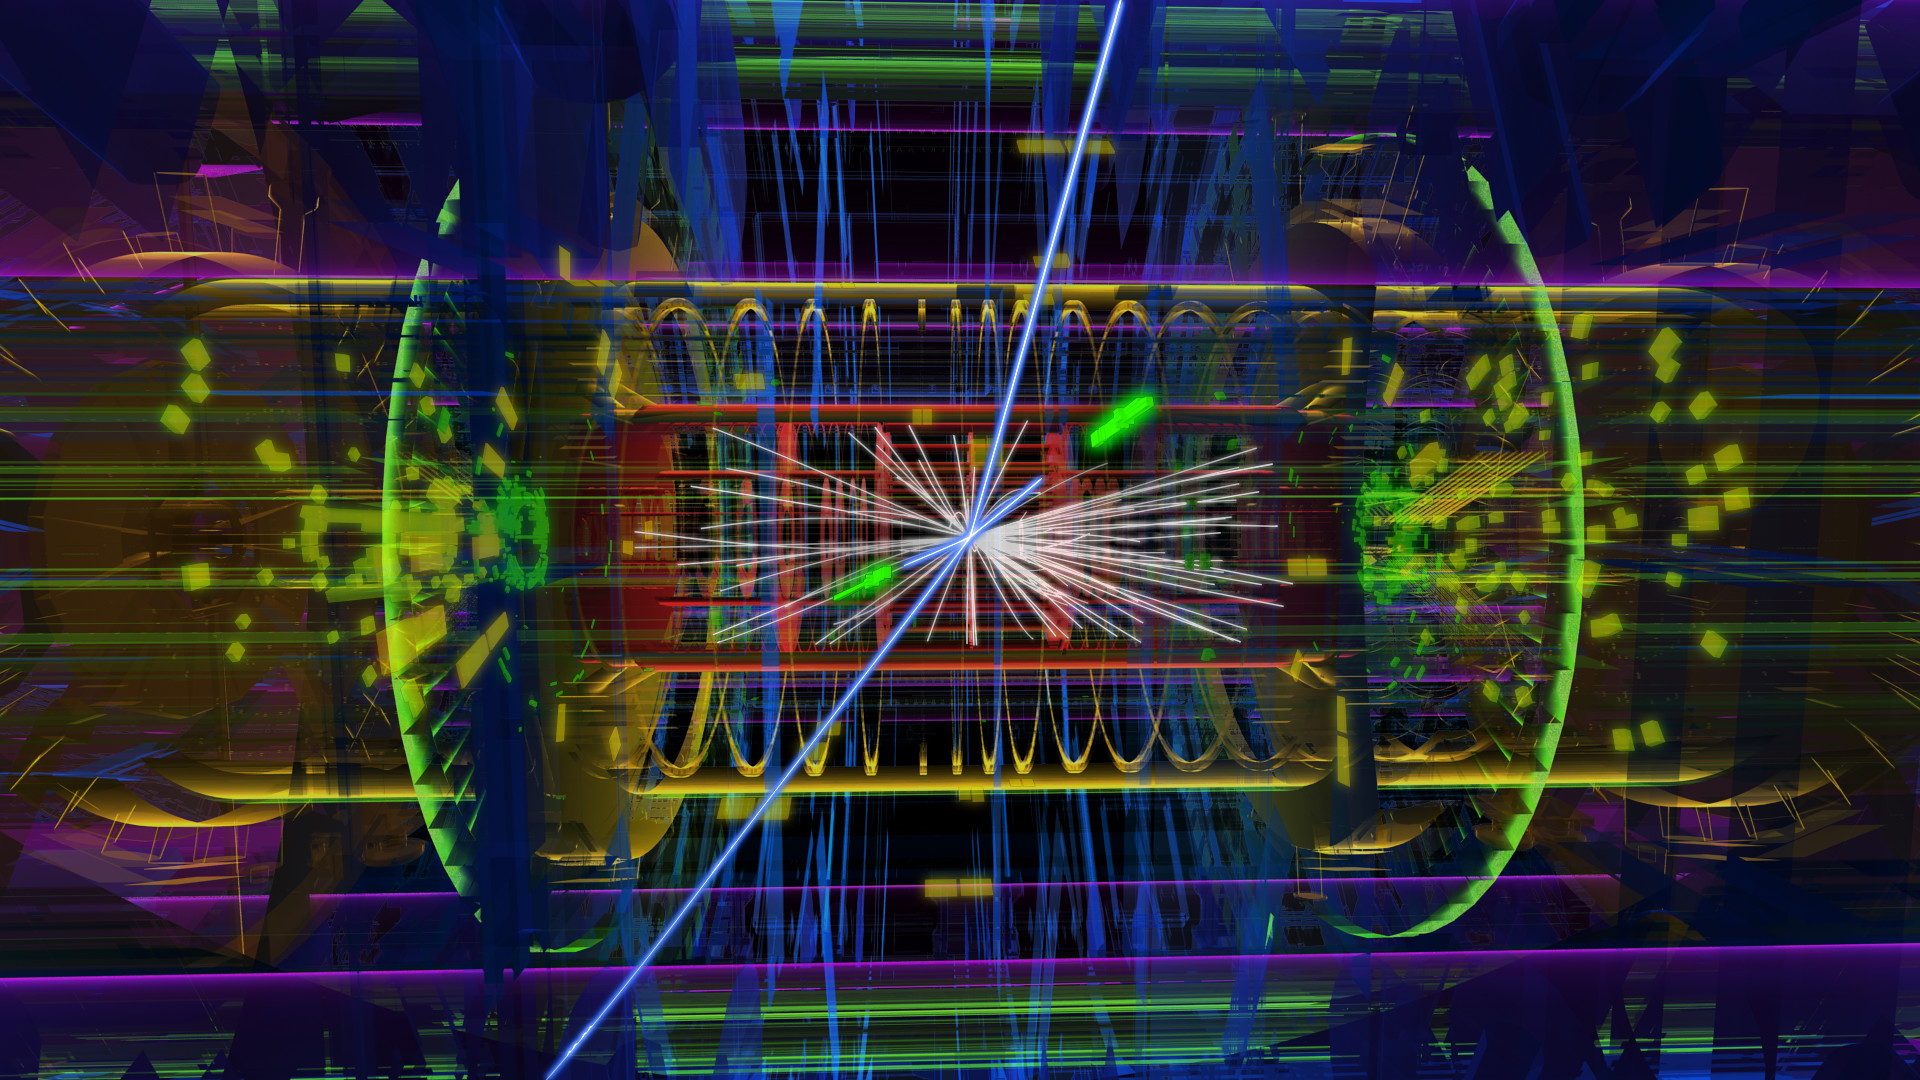
\includegraphics[height=1.2\textheight]{cern}};
      \end{tikzpicture}%
      }
\begin{poster}{
 % Show grid to help with alignment
 grid=false,
 % Column spacing
 colspacing=0.7em,
 % Color style
 headerColorOne=violet!90!white!50,
 borderColor=violet!90!white!50,
 % Format of textbox
 textborder=roundedsmall,
 % Format of text header
 headerborder=closed,
 headershape=roundedright,
 headershade=plain,
 background=user,
 %bgColorOne=white!100,
 boxshade = plain,
 headerheight=0.12\textheight
}
{
  \begin{tabular}{r}
    
\includegraphics[height=0.1\textheight]{inv}
  \end{tabular}
}
 % Title
 {\color{white} \sc{\Huge Numerical Solutions to Charmonium Wavefunctions}}
 % Authors
 {\color{white}
 {Matthew Rossetter}\\
 {Physics Problem Solving Computing Project}\\
 {Supervisor: Dr Ben Pecjak}\\
}
 % University logo
{
  \begin{tabular}{r}
    
\includegraphics[height=0.1\textheight]{logo0}
  \end{tabular}
 }

\headerbox{Introduction}{name=intro,column=0,row=0,span=2,boxColorOne=white}{
    Quarks are fundamental particles of the Standard Model of particle physics, most well-known for being the constituent particles of the proton and neutron. 
    They \textbf{cannot exist as free particles,} and so must be studied as part of bound systems.
    They can form quark-antiquark systems called quarkonium - these can be studied similarly to the Hydrogen atom, but using strong force interactions.
    The charm-anticharm system is known as Charmonium, and this will be the focus of this study.  
}

\headerbox{Theory}{name=theory,below=intro,column=0, span=1,boxColorOne=white}{
    The Charmonium wavefunction is found by solving the 3D Schrodinger equation \cite{qnl},
    \vspace{-10pt}
    \begin{align}
        -\frac{\hbar^2}{2\mu}\nabla^2\psi &+ [V(r) - E_{nl}]\psi = 0, \\
        V(r) &= -\frac{4\alpha_s}{3r} + \beta r.
        \vspace{-10pt}
    \end{align}
    Through separation of variables, $\psi = R_{nl}Y_l^m$, the radial wavefunction, $u_{nl} = rR_{nl}$, for each energy eigenvalue can be solved from a set of ODEs:
    \vspace{-10pt}
    \begin{align}
        \frac{du_{nl}}{dr} &= v_{nl} \\
        \frac{dv_{nl}}{dr} &= \frac{l(l+1)}{r^2}u_{nl} - 2\mu[E_{nl}-V(r)]u_{nl}
    \end{align}
    Boundary conditions must be set as $r\to0$. We set $u_{nl}(0) = 0$, and $\frac{du_{nl}}{dr} = 1$, ignoring normalisation until later.
    The program must start a small step away from the origin to compute non-zero solutions.
    The radial wavefunction must be normalised, such that
    \vspace{-10pt}
    \begin{equation}
        \int_0^{\infty} r^2|R_{nl}|^2\,dr = \int_0^\infty |u_{nl}|^2\,dr = 1.
    \end{equation}
}

\headerbox{The Bisection Method}{name=bis,below=theory,above=bottom,column=0,span=1,boxColorOne=white}{
    This method guesses three energies, $E_1, E_3$, and $E_2 = \frac{E_1+E_3}{2}$ to find $u_{nl}$.
    Using \texttt{scipy.integrate.odeint}, (3) and (4) are solved for these energies and normalised using Simpson's method. 
    The nodes and turning points are counted for each function - if these differ between two solutions, $E_{nl}$ lies somewhere between those energies. 
    \begin{figure}[H]
        \centering
        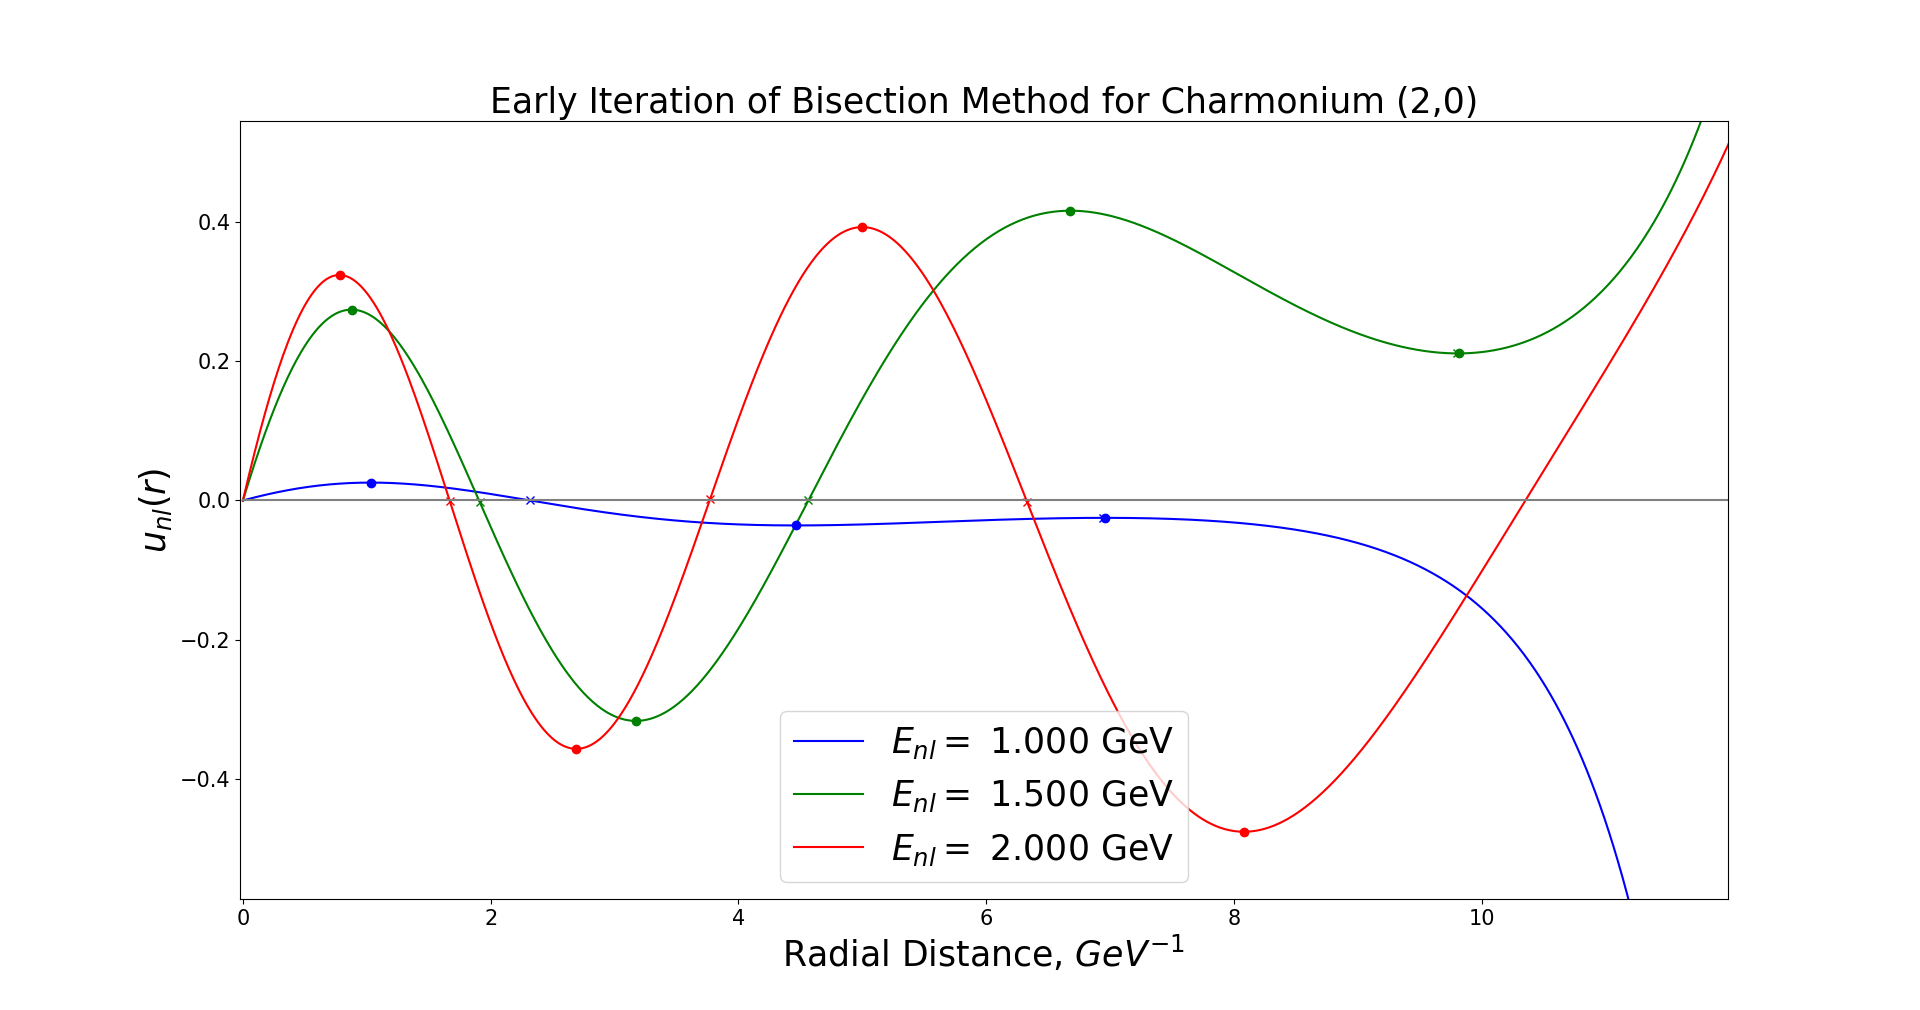
\includegraphics[width=0.85\linewidth]{nodes}
    \end{figure}
    \vspace{-5pt}
    $E_1$ and $E_3$ are set to the two energies over the difference, and $E_2$ calculated again. 
    We repeat this process until we find a correct $u_{nl}$, which has $(n-1)$ nodes and $n$ turning points. 
    The energy of this solution will be $E_{nl}$.
}

\headerbox{References}{name=references,column=2,span=2,above=bottom,boxColorOne=white}{
\nocite{*} % Print all references regardless of whether they were cited in the poster or not
\bibliographystyle{plain} % Plain referencing style
\bibliography{sample} % Use the example bibliography file sample.bib
}



\headerbox{The Hydrogen Wavefunction}{name=hydro,column=1,below=intro,span=1,boxColorOne=white}{
    To check the program is functioning for a simpler model, we apply it to the Hydrogen atom.
    The solution is found in the same way, with some constant changes:
    \begin{equation}
        \frac{4\alpha_s}{3} \to \alpha = \frac{1}{137},~ \beta \to 0,~ \mu \to m_e.
    \end{equation}
    Due to $l$-independence of the Hydrogen energies, for $l\neq0$ the number of nodes and turning points must be counted as $(n-l-1)$ and $(n-l)$ respectively.
    The program solved for $(n,l)=(1,0),(2,0),(2,1)$, with energies accurate to theory, and was then ready to move on to charmonium.
    \begin{figure}[H]
        \centering
        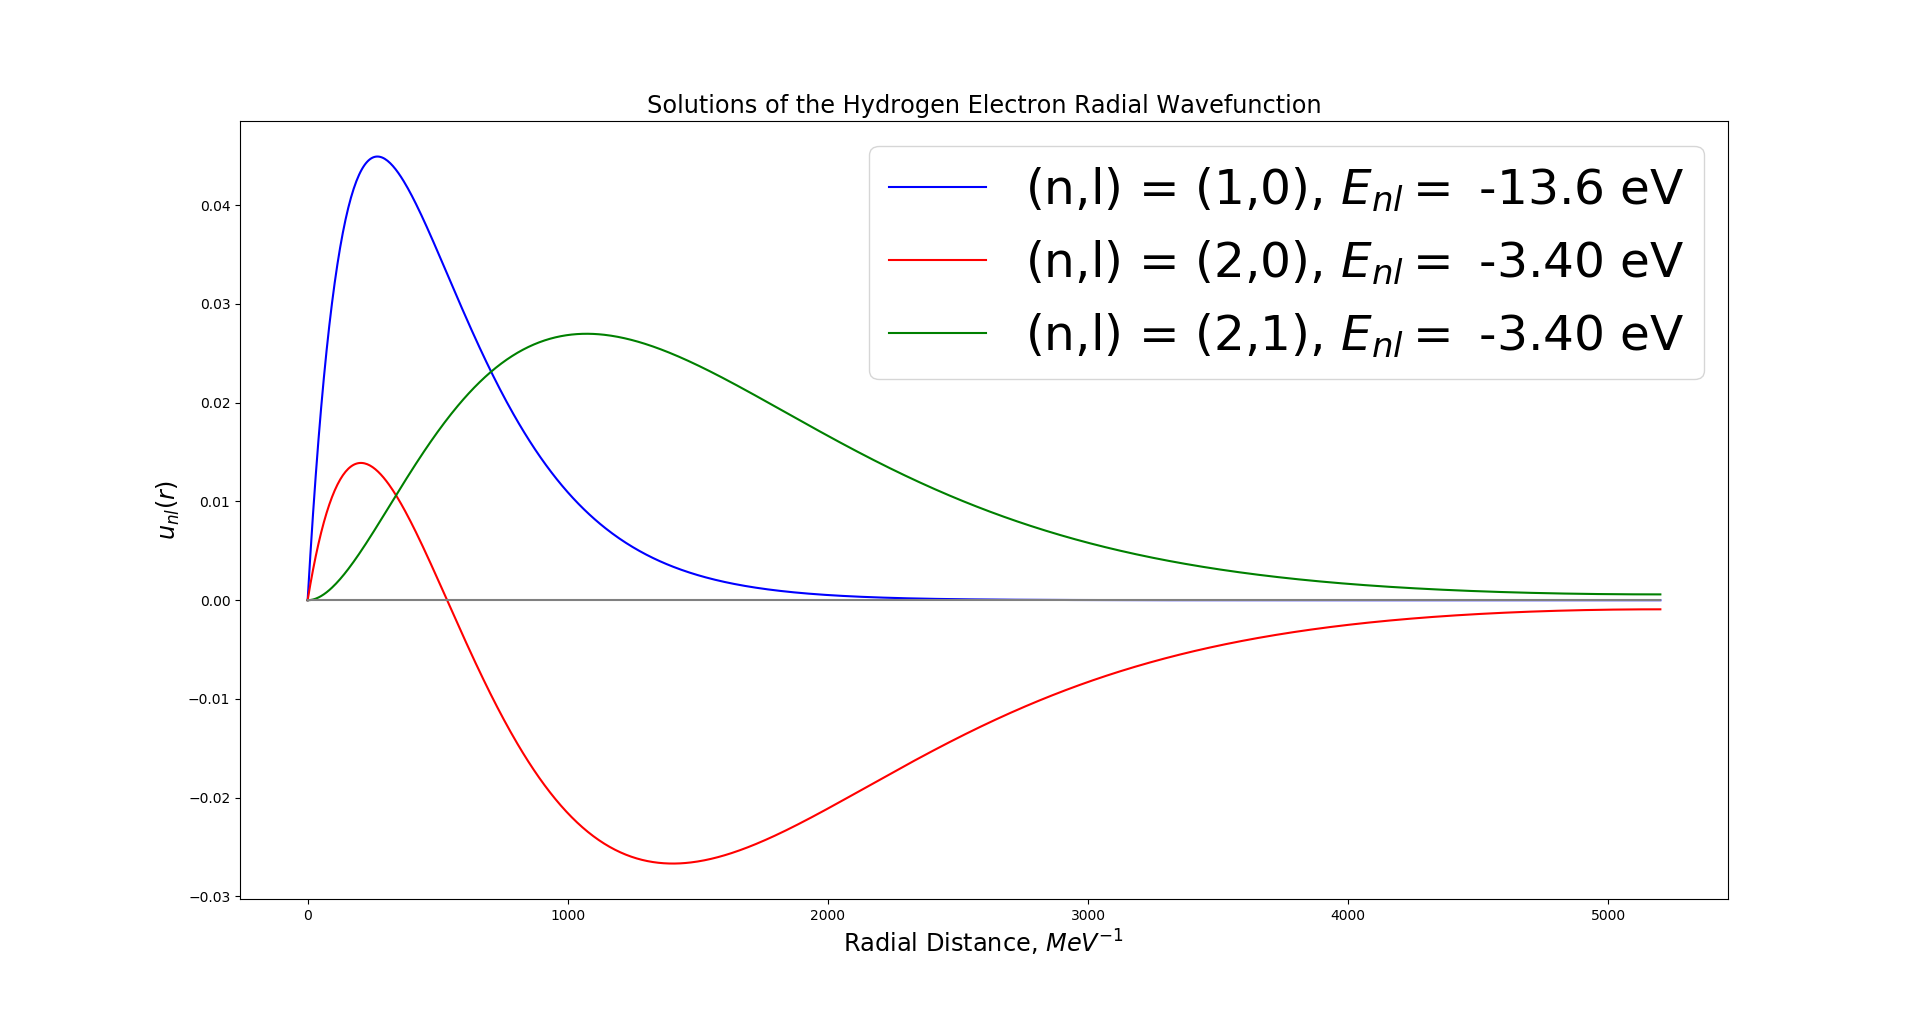
\includegraphics[width=\linewidth]{Hydro}
    \end{figure}
    \vspace{-20pt}
    \begin{align}
        E_{10} &= -13.6\,\text{eV} & E_{20} &= -3.40\,\text{eV} & E_{21} &= -3.40\,\text{eV}
    \end{align}
}

\headerbox{Calculating $\beta$}{name=beta,column=1,above=bottom,below=hydro,span=1,boxColorOne=white}{
    To solve the Charmonium wavefunction for any energy level, $\beta$ must first be known.
    The ground state energy is known through relation to the bound mass and charm quark mass:
   \vspace{-5pt}
    \begin{equation}
        M_{nl} = E_{nl} + 2m_c\,\cite{qnl},\, M_{nl} = 3.068\text{Gev}/c^2,~ m_c = 1.34\text{GeV}/c^2 
    \end{equation}
    The bisection method is performed over $\beta$ with ground state energy a constant, and $\beta$'s value is found.
    \begin{figure}[H]
        \centering
        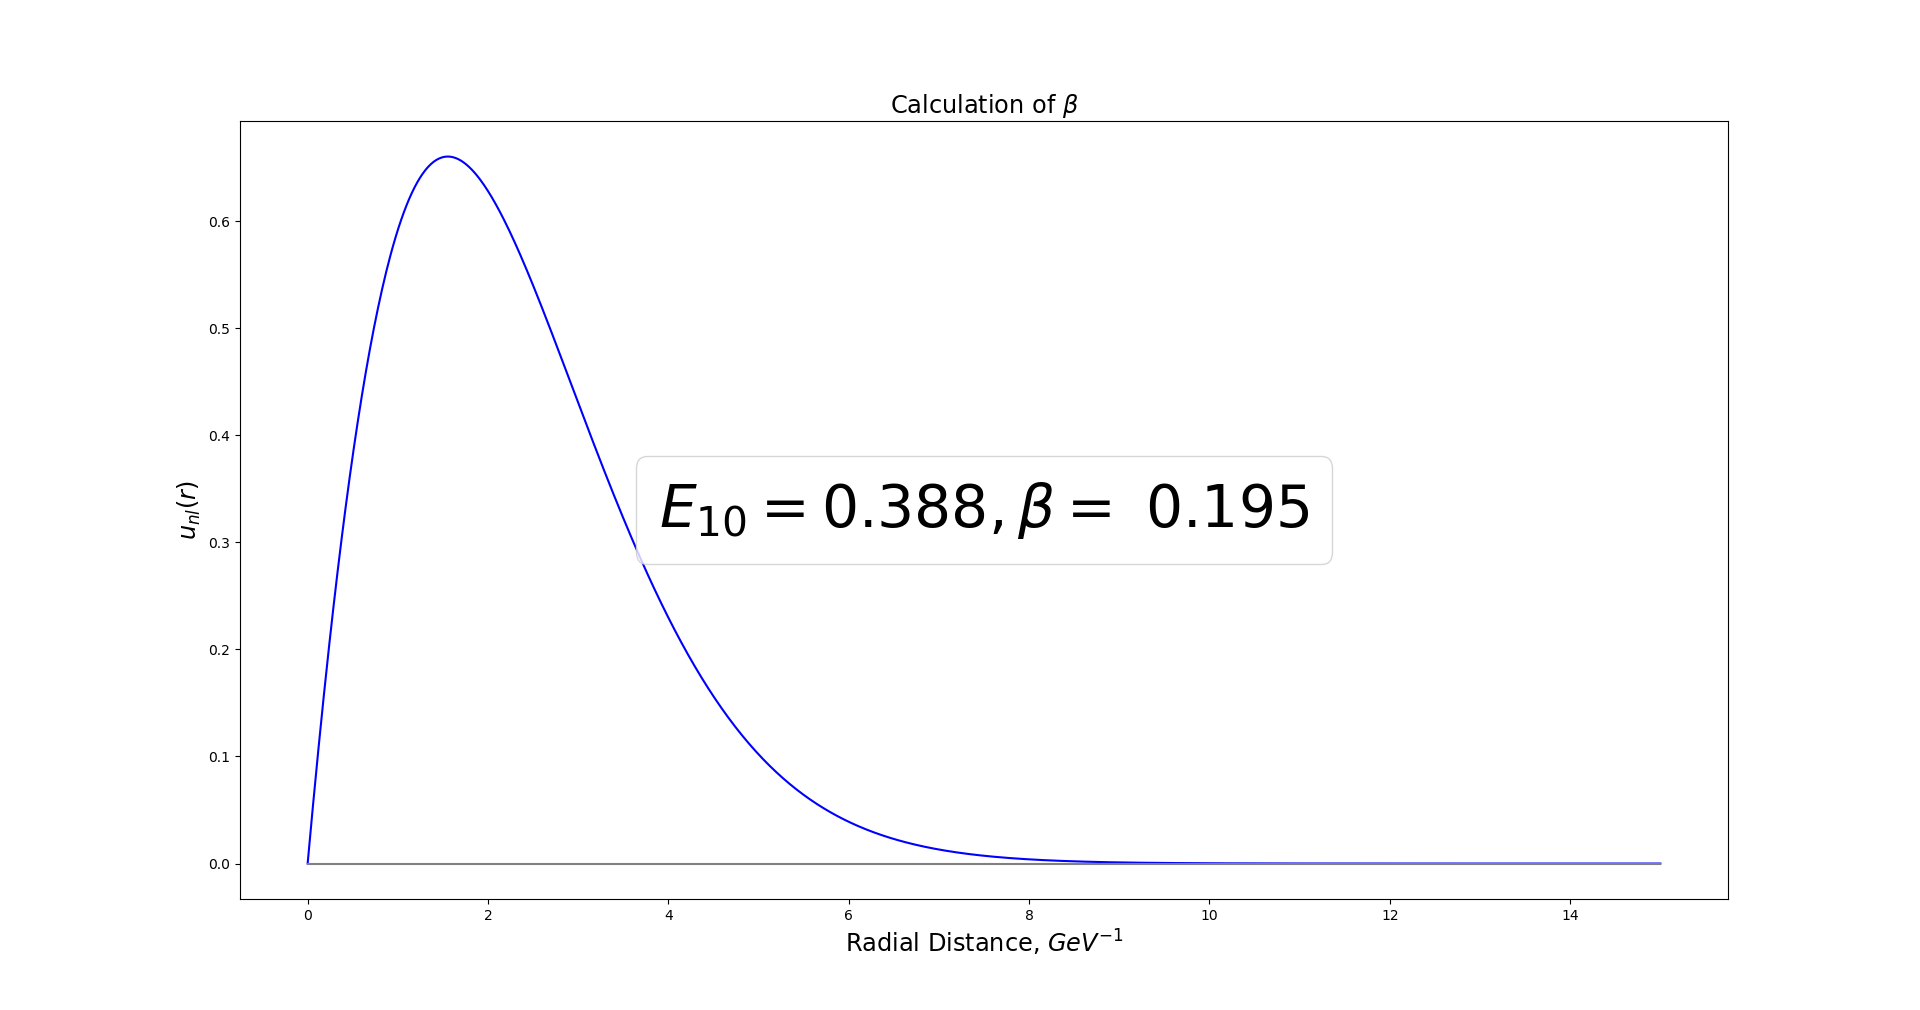
\includegraphics[width=0.9\linewidth]{beta}
    \end{figure}
}

\headerbox{Finding the Charmonium Wavefunctions}{name=comp,above=references,column=2,span=1,boxColorOne=white}{
    With a known value of $\beta = 0.195$, we can proceed to solve the Charmonium wavefunction, with the strong coupling constant,
    \begin{equation}
        \alpha_s = 0.4.
    \end{equation}
    We can check that this value of $\beta$ yields the correct energy for the ground state of Charmonium, and then apply it to the (1,1) and (2,0) states as well to find their energies. 
    Now using the same method as before, having confirmed the functionality of the program on hydrogen, the solutions of the radial wavefunction are solved.

    Without examining the results of computations, it can be seen that the nodes and turning points cannot depend on the value of $l$, as seen in Hydrogen, if the (1,1) state is to have a non-zero wavefunction. 
    So we go back to the original $(n-1)$ nodes and $n$ turning points method original stated for the bisection method.
    \begin{figure}[H]
        \centering
        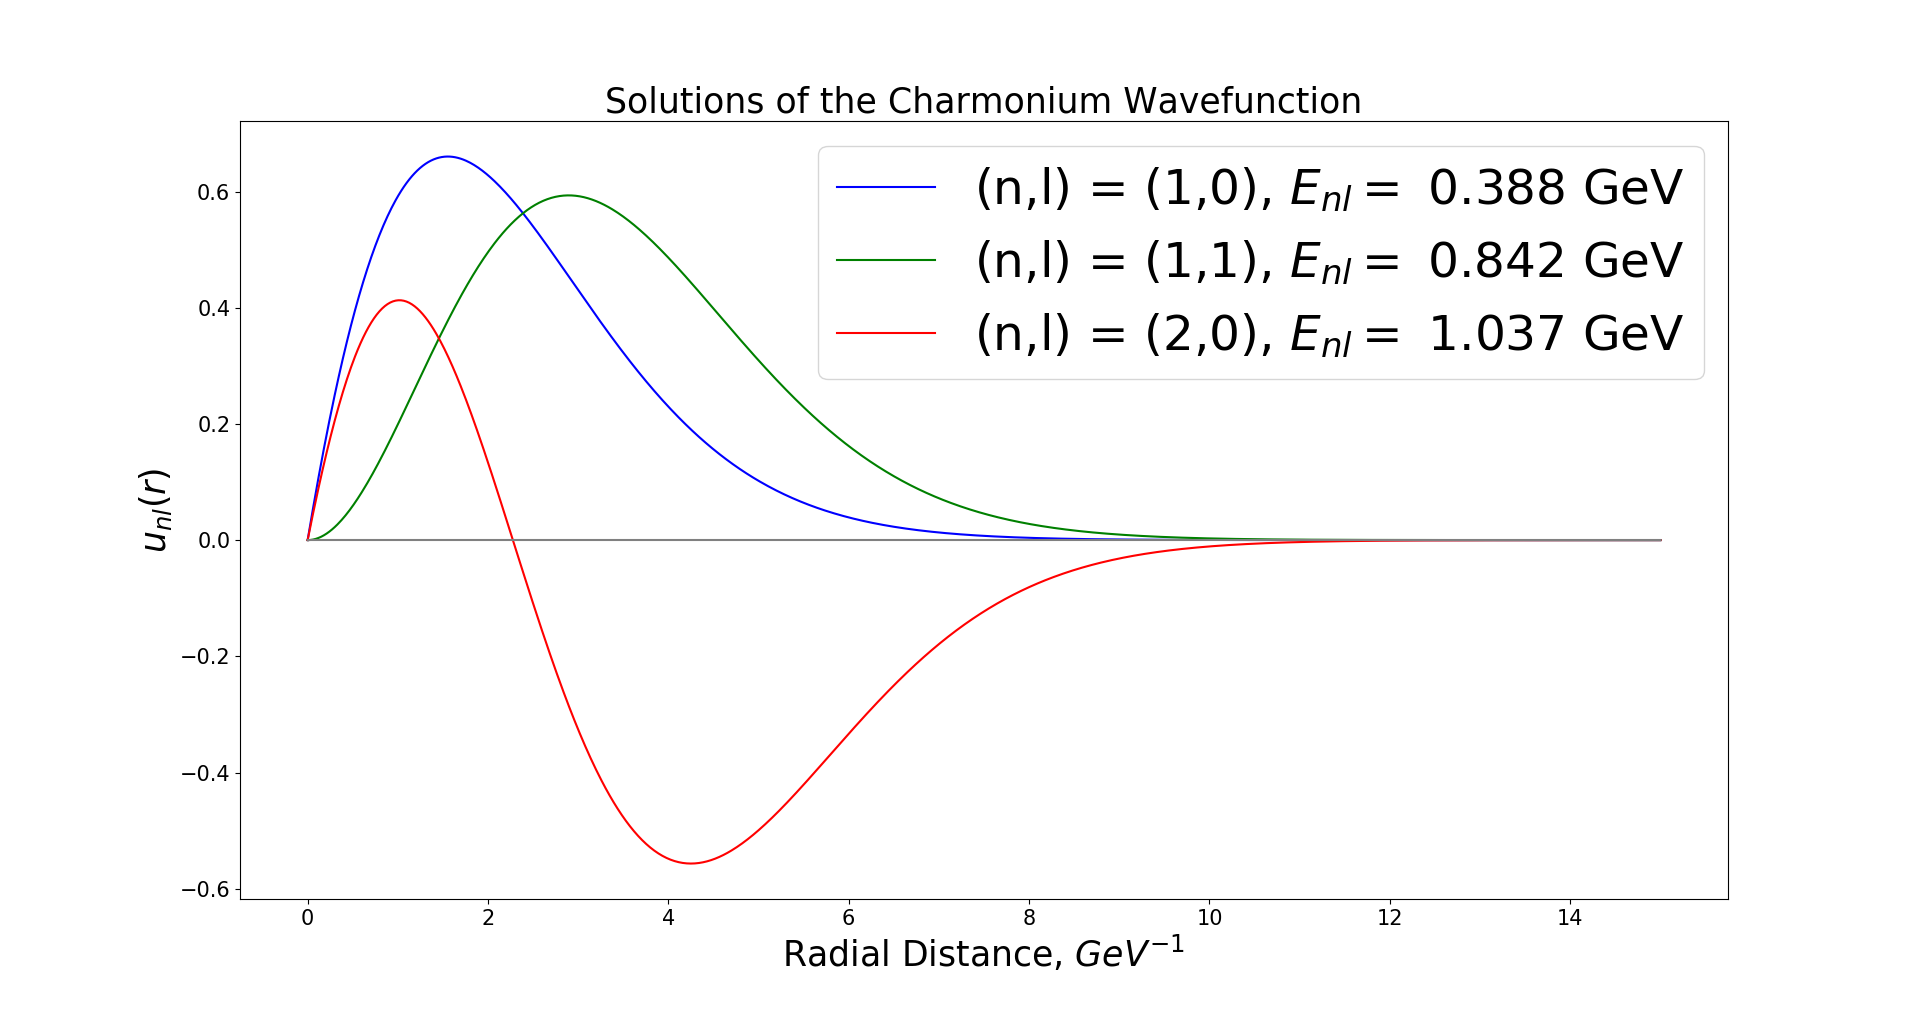
\includegraphics[width=\linewidth]{Charmonium}
    \end{figure}
    \vspace{-15pt}
    \begin{align}
        E_{10} &= 0.388\,\text{GeV} & E_{11} &= 0.842\,\text{GeV} & E_{20} &= 1.037\,\text{GeV}
    \end{align}
    From these results, it is obvious that, unlike the hydrogen atom, the energy of the system depends on both the $n$ and $l$ quantum numbers, instead of just the $n$.\\
    These energies can then be checked against theory by converting to bound masses through (8) and compared to values for each state given in \cite{website:pdg}. \\
    The ground state bound mass and charm mass were given values to be used at the beginning of this project, differing from results in \cite{website:pdg} due to spin-averaging.
    The (1,1) and (2,0) states calculated have energies broadly accurate with the spin-average of states given in \cite{website:pdg} - the difference comes from hyperfine splitting which has not yet been considered, but the average energy of the states roughly agrees with expectations.
}

\headerbox{Outlook}{name=outlook,column=3,span=1,boxColorOne=white}{
    Now with a functioning program, further extensions to the study can be considered. 
    The energies of the states were seen to be somewhat innacurate to the known measurements, at least partially due to the hyperfine spin interactions which causes a splitting in the energy \cite{qnl}.
    This splitting is
    \vspace{-10pt}
    \begin{equation}
        \Delta(n^3S_1 - n_1S_0) = \frac{8\alpha_s}{9m_q^2}|R_{nl}(0)|^2,
    \end{equation}
    so the energies calculated in this project will be the spin-average of the hyperfine energies, to be tested in further studies.
    The splitting depends on the value of the wavefunction at $r=0$, which is
    \vspace{-10pt}
    \begin{equation}
        \lim_{r\to0} R_{nl}(r) = \lim_{r\to0} \frac{u_{nl}(r)}{r} = \frac{du_{nl}(0)}{dr}.
    \end{equation}
    Transition rates between these states can be studied to give further insight into the strong force.
}

\headerbox{Faults of the Method}{name=faults,column=3, above=references, below=outlook, boxColorOne=white}{
    \textbf{Choice of Energy:} 
    If the energy eigenvalue does not lie within the range of the initial guess for energy, then the program will not be able to solve for it, so using this program requires some vague knowledge of where the energy will lie.\\
    \textbf{Tolerances:}
    The program requires fine tuning of tolerance levels testing for the convergence of the energies. 
    If the tolerance is too high or too low, the energy will be slightly too high or low and the function will diverge to infinity. 
    \begin{figure}[H]
        \centering
        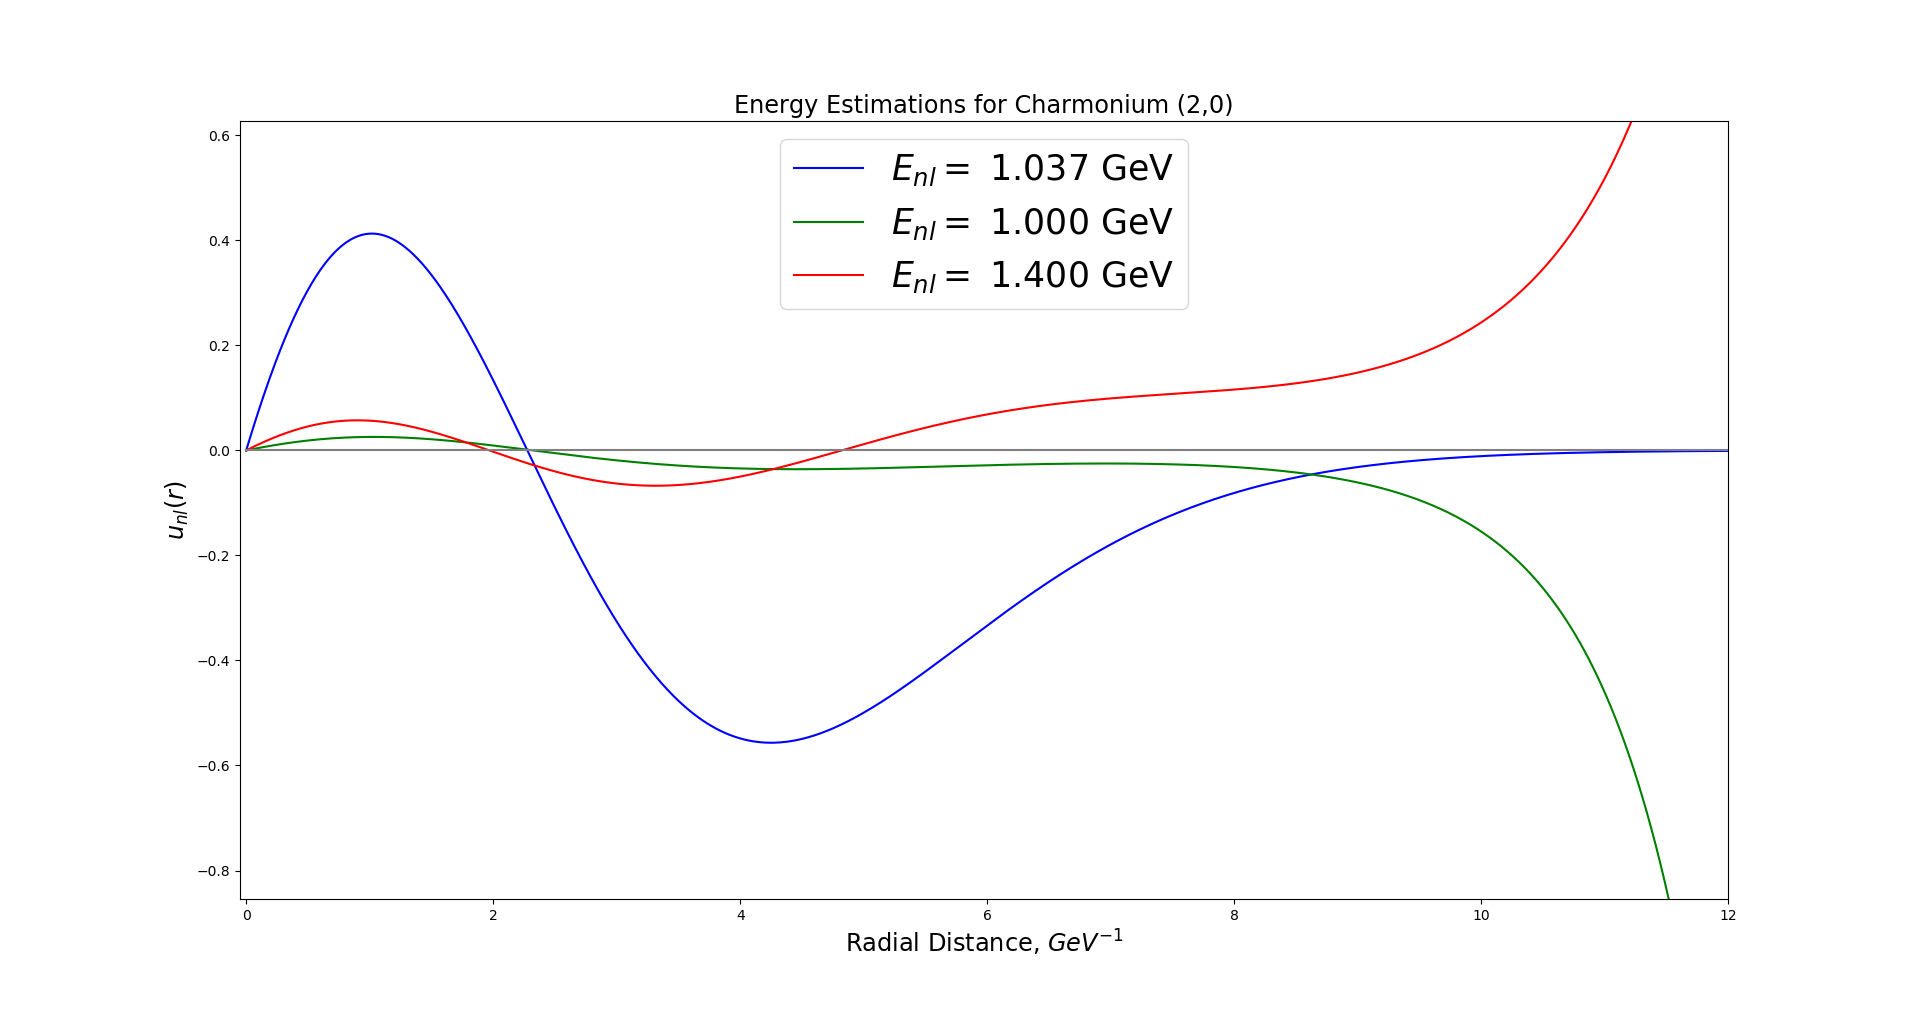
\includegraphics[width=0.9\linewidth]{div}
    \end{figure}
    \vspace{-5pt}
    \textbf{Initial Values:}
    The program can only be as accurate as the initial values put in. 
    If the values of mass, and $\alpha_s$, they will result in different end results for energy. 
    Thus, comparison to known values can only be valid if these parameters are approximately similar.
    The values were also spin-averaged, so considering hyperfine splitting will change results.
}
\end{poster}%
%
\end{document}
